Let $m, k \in \NN$  and $\epsilon \in (0,1]$. 
Let $w$ be a characteristic string of length $T = m + k$ such that 
the bits of $w$ are i.i.d.\ Bernoulli with expectation $\alpha = (1 - \epsilon)/2$. 
Write $w$ as $w = xy$ where $|x| = m, |y| = k$.
% where 
% each bit is independent with $\Pr[w_i = 1] = \alpha$.
The recursive definition of relative margin (cf. Lemma~\ref{lem:relative-margin}) 
implies an algorithm for computing the probability
$\Pr[\mu_x(y) \geq 0]$ in time $\Poly(m, k)$. In typical
circumstances, however, it is more interesting to establish an
explicit upper bound on $\Pr[\mu_x(y) \geq 0]$ where
$|x| \rightarrow \infty$; this corresponds to the case where the
distribution of the initial reach $\rho(x)$ is the dominant distribution
$\StationaryRho$ in Lemma~\ref{lemma:rho-stationary}. 
Due to dominance, $\StationaryRho(m)$ serves as an
upper bound on $\rho(x)$ for any finite $m = |x|$. 
For this purpose, one can implicitly
maintain a sequence of matrices $\left( M_t \right)$ for $t = 0, 1, 2, \cdots, k$
such that $M_0(r, r) = \StationaryRho(r)$ for all $0 \leq r \leq 2k$ and
the invariant
\[
  M_t(r, s) = \Pr_{y \sim \mathcal{B}(t, \alpha)}[\rho(xy) = r \text{ and }
  \mu_x(y) = s ]
\]
is satisfied for every integer $t \in [1, k]$,
$r \in [0, 2k]$, and $s \in [-2k, 2k]$. 
Here, $M(i,j)$ denotes the entry at the $i$th row and $j$th column of the matrix $M$.
%The matrix $M_0$ corresponds to the reach and margin after any prefix $x$. 
Observe that $M_t(r,s)$ can be computed solely from the neighboring cells of $M_{t-1}$, that is, 
from the values $M_{t-1}(r\pm 1, s \pm 1)$. 
Of course, only the transitions approved by the recursions in 
Lemma~\ref{lem:margin} and Lemma~\ref{lem:relative-margin} should be considered.

Finally, one can compute $\Pr[\mu_x(y) \geq 0]$ by summing $M_k(r,s)$ for
$r, s \geq 0$. Table~\ref{table:exact-probs} contains these
probabilities where $\alpha$ ranges from $0.05$ to $0.40$ and $k$
ranges from $50$ to $1000$. 
In addition, Figure~\ref{fig:exact-probs} shows the base-$10$ logarithm of
these probabilities. The
points corresponding to a fixed $\alpha$ appear to form a straight
line. This means the probability decays exponentially in $k$, or equivalently, that the exponent 
depends linearly on $k$, 
as stipulated by Bound~\ref{bound:analytic}. 

A \texttt{C++} implementation of the above algorithm is publicly available 
at: \\
\href{https://github.com/saad0105050/forkable-strings-code}{https://github.com/saad0105050/forkable-strings-code}~\cite{PrForkableCode}.



\begin{figure}[h!]

\centering
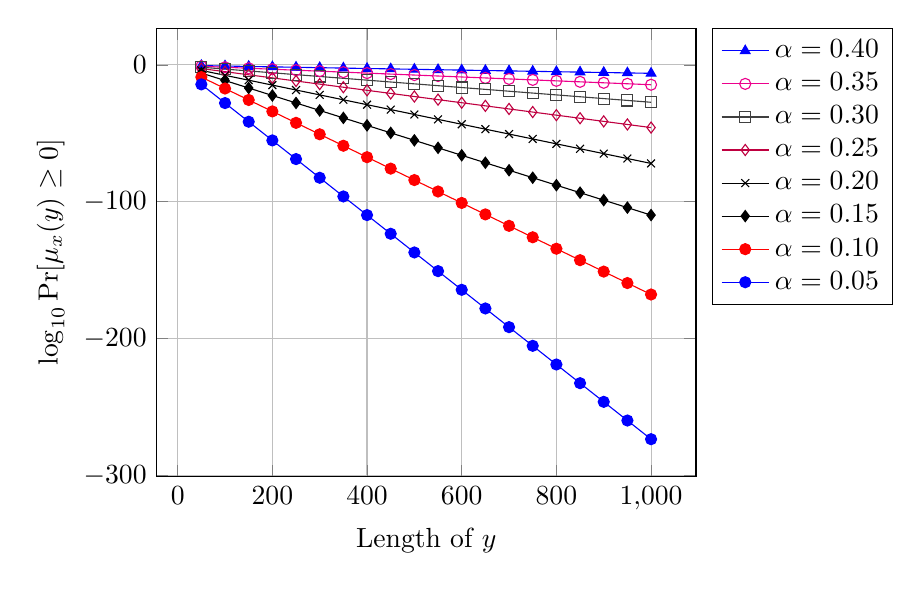
\begin{tikzpicture}
  \begin{axis}[
    xlabel=Length of $y$,
    ylabel=${\log_{10} \Pr[ \mu_x(y) \geq 0 ]}$,
    legend pos = outer north east,
    grid = both
    %,height = 7cm
    ]


    %============= \alpha = 0.40    
      \addplot[color=blue,mark=triangle*] coordinates {
    (50, -0.534881009996625)
    (100, -0.861843437303938)
    (150, -1.17110438398993)
    (200, -1.47350880258986)
    (250, -1.77251864117173)
    (300, -2.06962896433787)
    (350, -2.36559449154758)
    (400, -2.66083495643829)
    (450, -2.95559969289654)
    (500, -3.25004400806221)
    (550, -3.54426813580273)
    (600, -3.83833855715903)
    (650, -4.1323003235163)
    (700, -4.42618449355664)
    (750, -4.72001278023346)
    (800, -5.01380053810684)
    (850, -5.30755872931896)
    (900, -5.60129524293208)
    (950, -5.89501579493968)
    (1000, -6.18872455077118)


      };
      
    %============= \alpha = 0.35    
      \addplot[color=magenta,mark=o] coordinates {
    (50, -1.02877436841824)
    (100, -1.76405795532126)
    (150, -2.48156081504761)
    (200, -3.19351655688251)
    (250, -3.90324719739329)
    (300, -4.6119732073238)
    (350, -5.32021396523135)
    (400, -6.0282101484992)
    (450, -6.73607948155516)
    (500, -7.44388168223398)
    (550, -8.15164782799613)
    (600, -8.85939439475358)
    (650, -9.56713023906372)
    (700, -10.2748601722391)
    (750, -10.9825868295165)
    (800, -11.6903116636224)
    (850, -12.3980354795589)
    (900, -13.1057587252749)
    (950, -13.8134816508858)
    (1000, -14.521204396449)  


      };

    %============= \alpha = 0.30    
        \addplot[color=darkgray,mark=square] coordinates {
    (50, -1.73119438208806)
    (100, -3.09673279902966)
    (150, -4.44780375955355)
    (200, -5.79553003490465)
    (250, -7.14227457376805)
    (300, -8.48869966525932)
    (350, -9.83501495946096)
    (400, -11.1812912676285)
    (450, -12.5275534426098)
    (500, -13.873810422115)
    (550, -15.2200654730463)
    (600, -16.5663198030557)
    (650, -17.9125738621863)
    (700, -19.258827819142)
    (750, -20.6050817374433)
    (800, -21.9513356410858)
    (850, -23.2975895391646)
    (900, -24.6438434351249)
    (950, -25.9900973302771)
    (1000, -27.3363512251228)  


      };



    %============= \alpha = 0.25    
      \addplot[color=purple,mark=diamond] coordinates {
    (50, -2.7068067143968)
    (100, -4.98669572210932)
    (150, -7.25681899248793)
    (200, -9.52547099796917)
    (250, -11.793848036259)
    (300, -14.0621691284583)
    (350, -16.3304783495448)
    (400, -18.5987849921223)
    (450, -20.8670910667017)
    (500, -23.1353970150404)
    (550, -25.4037029351594)
    (600, -27.6720088489442)
    (650, -29.9403147613032)
    (700, -32.2086206733433)
    (750, -34.4769265853085)
    (800, -36.7452324972576)
    (850, -39.0135384092045)
    (900, -41.281844321149)
    (950, -43.5501502330935)
    (1000, -45.8184561450381)


      };


          
    %============= \alpha = 0.    
      \addplot[color=black,mark=x] coordinates {
    (50, -4.06125884952046)
    (100, -7.64248504871986)
    (150, -11.2184152058828)
    (200, -14.7939108371324)
    (250, -18.3693634087138)
    (300, -21.9448114175389)
    (350, -25.520258928049)
    (400, -29.095706383289)
    (450, -32.6711538323473)
    (500, -36.2466012807114)
    (550, -39.822048728996)
    (600, -43.3974961772738)
    (650, -46.9729436255496)
    (700, -50.5483910738248)
    (750, -54.1238385221004)
    (800, -57.6992859703754)
    (850, -61.2747334186509)
    (900, -64.8501808669272)
    (950, -68.4256283152027)
    (1000, -72.0010757634778)




      };
      
    %============= \alpha = 0.15    
      \addplot[color=black,mark=diamond*] coordinates {
    (50, -5.99101535930985)
    (100, -11.4538646368115)
    (150, -16.9145865673508)
    (200, -22.3752357117723)
    (250, -27.8358819361379)
    (300, -33.2965280374903)
    (350, -38.7571741335604)
    (400, -44.2178202294009)
    (450, -49.6784663252318)
    (500, -55.1391124210625)
    (550, -60.5997585168932)
    (600, -66.0604046127235)
    (650, -71.5210507085538)
    (700, -76.9816968043839)
    (750, -82.4423429002152)
    (800, -87.9029889960452)
    (850, -93.3636350918761)
    (900, -98.8242811877078)
    (950, -104.284927283538)
    (1000, -109.745573379367)


    };


    %============= \alpha = 0.10    
      \addplot[color=red,mark=*] coordinates {
    (50, -8.93400016060089)
    (100, -17.292337808078)
    (150, -25.6501551609344)
    (200, -34.007967886374)
    (250, -42.3657805652942)
    (300, -50.7235932437328)
    (350, -59.0814059221663)
    (400, -67.4392186006004)
    (450, -75.7970312790341)
    (500, -84.1548439574669)
    (550, -92.5126566359009)
    (600, -100.870469314334)
    (650, -109.228281992768)
    (700, -117.586094671201)
    (750, -125.943907349634)
    (800, -134.301720028069)
    (850, -142.659532706502)
    (900, -151.017345384936)
    (950, -159.375158063369)
    (1000, -167.732970741802)



    };
    %============= \alpha = 0.05    
      \addplot[color=blue,mark=*] coordinates {
    (50, -14.2699842004544)
    (100, -27.9093384792564)
    (150, -41.5486518624197)
    (200, -55.1879652167995)
    (250, -68.8272785711567)
    (300, -82.4665919255127)
    (350, -96.10590527987)
    (400, -109.745218634226)
    (450, -123.384531988584)
    (500, -137.023845342941)
    (550, -150.663158697297)
    (600, -164.302472051655)
    (650, -177.94178540601)
    (700, -191.581098760368)
    (750, -205.220412114725)
    (800, -218.859725469083)
    (850, -232.499038823439)
    (900, -246.138352177796)
    (950, -259.777665532154)
    (1000, -273.41697888651)

 
  };
  \legend{
  $\alpha = 0.40$, $\alpha = 0.35$, 
   $\alpha = 0.30$,$\alpha = 0.25$, $\alpha = 0.20$, 
   $\alpha = 0.15$,$\alpha = 0.10$,  $\alpha = 0.05$
  }
  \end{axis}%
\end{tikzpicture}%
\caption{The probabilities from Table~\ref{table:exact-probs}  
drawn in the base-$10$ logarithmic scale. 
}
\label{fig:exact-probs}
\end{figure}





%%%%% If dissertation, display table in landscape mode
\iftoggle{Dissertation}{
  \begin{landscape}
}

\begin{table}[h]
	\centering
	\caption[Exact settlement error probabilities for Boolean characteristic strings]{
		Exact probabilities $\Pr[\mu_x(y) \geq 0]$ where 
		the bits of the characteristic string $xy$ are i.i.d.\ Bernoulli with expectation $\alpha$. 
		Each row of the table corresponds to a different $k = |y|$.
	} 
	\label{table:exact-probs}


	\begin{tabular}{|l||l|l|l|l|l|l|l|l|}
	\hline
	\multicolumn{1}{|c||}{\multirow{2}{*}{$k$}} & \multicolumn{8}{c|}{$\alpha$}                                             \\ \cline{2-9} 
	\multicolumn{1}{|c||}{}                   & 0.05     & 0.10      & 0.15     & 0.20      & 0.25     & 0.30      & 0.35     & 0.40      \\ 
	\hhline{|=#=|=|=|=|=|=|=|=|}
	50   & 5.37E-15  & 1.16E-09  & 1.02E-06  & 8.68E-05 & 1.96E-03 & 1.86E-02 & 9.36E-02 & 2.92E-01 \\ \hline
	100  & 1.23E-28  & 5.10E-18  & 3.52E-12  & 2.28E-08 & 1.03E-05 & 8.00E-04 & 1.72E-02 & 1.37E-01 \\ \hline
	150  & 2.83E-42  & 2.24E-26  & 1.22E-17  & 6.05E-12 & 5.54E-08 & 3.57E-05 & 3.30E-03 & 6.74E-02 \\ \hline
	200  & 6.49E-56  & 9.82E-35  & 4.21E-23  & 1.61E-15 & 2.98E-10 & 1.60E-06 & 6.40E-04 & 3.36E-02 \\ \hline
	250  & 1.49E-69  & 4.31E-43  & 1.46E-28  & 4.27E-19 & 1.61E-12 & 7.21E-08 & 1.25E-04 & 1.69E-02 \\ \hline
	300  & 3.42E-83  & 1.89E-51  & 5.05E-34  & 1.14E-22 & 8.67E-15 & 3.25E-09 & 2.44E-05 & 8.52E-03 \\ \hline
	350  & 7.84E-97  & 8.29E-60  & 1.75E-39  & 3.02E-26 & 4.67E-17 & 1.46E-10 & 4.78E-06 & 4.31E-03 \\ \hline
	400  & 1.80E-110 & 3.64E-68  & 6.06E-45  & 8.02E-30 & 2.52E-19 & 6.59E-12 & 9.37E-07 & 2.18E-03 \\ \hline
	450  & 4.13E-124 & 1.60E-76  & 2.10E-50  & 2.13E-33 & 1.36E-21 & 2.97E-13 & 1.84E-07 & 1.11E-03 \\ \hline
	500  & 9.47E-138 & 7.00E-85  & 7.26E-56  & 5.67E-37 & 7.32E-24 & 1.34E-14 & 3.60E-08 & 5.62E-04 \\ \hline
	550  & 2.17E-151 & 3.07E-93  & 2.51E-61  & 1.51E-40 & 3.95E-26 & 6.02E-16 & 7.05E-09 & 2.86E-04 \\ \hline
	600  & 4.98E-165 & 1.35E-101 & 8.70E-67  & 4.00E-44 & 2.13E-28 & 2.71E-17 & 1.38E-09 & 1.45E-04 \\ \hline
	650  & 1.14E-178 & 5.91E-110 & 3.01E-72  & 1.06E-47 & 1.15E-30 & 1.22E-18 & 2.71E-10 & 7.37E-05 \\ \hline
	700  & 2.62E-192 & 2.59E-118 & 1.04E-77  & 2.83E-51 & 6.19E-33 & 5.51E-20 & 5.31E-11 & 3.75E-05 \\ \hline
	750  & 6.02E-206 & 1.14E-126 & 3.61E-83  & 7.52E-55 & 3.33E-35 & 2.48E-21 & 1.04E-11 & 1.91E-05 \\ \hline
	800  & 1.38E-219 & 4.99E-135 & 1.25E-88  & 2.00E-58 & 1.80E-37 & 1.12E-22 & 2.04E-12 & 9.69E-06 \\ \hline
	850  & 3.17E-233 & 2.19E-143 & 4.33E-94  & 5.31E-62 & 9.69E-40 & 5.04E-24 & 4.00E-13 & 4.93E-06 \\ \hline
	900  & 7.27E-247 & 9.61E-152 & 1.50E-99  & 1.41E-65 & 5.23E-42 & 2.27E-25 & 7.84E-14 & 2.50E-06 \\ \hline
	950  & 1.67E-260 & 4.22E-160 & 5.19E-105 & 3.75E-69 & 2.82E-44 & 1.02E-26 & 1.54E-14 & 1.27E-06 \\ \hline
	1000 & 3.83E-274 & 1.85E-168 & 1.80E-110 & 9.98E-73 & 1.52E-46 & 4.61E-28 & 3.01E-15 & 6.48E-07 \\ \hline
	\end{tabular}

\end{table}
%%%%% If dissertation, display table in landscape mode
\iftoggle{Dissertation}{
  \end{landscape}
}



%%% Local Variables:
%%% mode: latex
%%% TeX-master: "main"
%%% End:
